\documentclass[11pt,a4paper]{article}
\usepackage[margin=1in]{geometry}
\usepackage{calc}
\usepackage{array}
\usepackage{graphicx}
\usepackage{fancyhdr}
\usepackage[hidelinks]{hyperref}
\usepackage{url}
\graphicspath{../}
\usepackage{float}
\usepackage{listings}
\usepackage{threeparttable}

\usepackage{tikz}
\usetikzlibrary{shapes, arrows, decorations.markings, positioning}

\usepackage{cleveref} 

% Break URL on hyphens
\makeatletter
\g@addto@macro{\UrlBreaks}{\UrlOrds}
\makeatother

\pagestyle{fancy}
\fancyhf{}
\renewcommand{\headrulewidth}{0pt} % Remove line
\fancyfoot[R]{Version \input{|"git rev-parse --short HEAD"}}
\fancyhead[C]{\leftmark}
\fancyfoot[L]{\thepage}

\setlength{\parindent}{0cm}  % No indent on pararaph

\newlength\myheight
\newlength\mydepth
\settototalheight\myheight{Xygp}
\settodepth\mydepth{Xygp}
\setlength\fboxsep{0pt}
\newcommand*\inlinegraphics[1]{%
  \settototalheight\myheight{Xygp}%
  \settodepth\mydepth{Xygp}%
  \raisebox{-\mydepth}{\includegraphics[height=\myheight]{#1}}%
}

\newcommand{\instructionbox}[2]{\medskip%
\fbox{\begin{minipage}{\textwidth}%
    \medskip%
    \begin{center}%
        #1%
    \end{center}%
    \medskip%
\end{minipage}}%
\medskip%
}

\usepackage{xcolor}
 
\definecolor{codegreen}{rgb}{0,0.6,0}
\definecolor{codegray}{rgb}{0.5,0.5,0.5}
\definecolor{codepurple}{rgb}{0.58,0,0.82}
\definecolor{backcolour}{rgb}{0.95,0.95,0.92}
 
\lstdefinestyle{mystyle}{
    backgroundcolor=\color{backcolour},   
    commentstyle=\color{codegreen},
    keywordstyle=\color{magenta},
    numberstyle=\tiny\color{codegray},
    stringstyle=\color{codepurple},
    basicstyle=\ttfamily\footnotesize,
    breakatwhitespace=false,         
    breaklines=true,                 
    captionpos=b,                    
    keepspaces=true,                 
    numbers=left,                    
    numbersep=5pt,                  
    showspaces=false,                
    showstringspaces=false,
    showtabs=false,                  
    tabsize=4
}
\lstset{style=mystyle}

\newcommand{\handwaving}{\inlinegraphics{./src/hand.png}}

\title{VHDL 101}
\author{Patrick Mintram}

\begin{document}

\clearpage\maketitle
\thispagestyle{empty} % No page numbering
\pagebreak

\section{Intoduction}
Things this session is intended to wet your appetite to the world of FPGAs, so that if you choose to you can start having a play in your own time. This session is:
\begin{enumerate}
    \item A brief overview of VHDL
    \item A chance to get hands on with some Hardware
    \item A chance to make a \texttt{hello world} in Hardware
\end{enumerate}

Things this session is \emph{not}:
\begin{enumerate}
    \item An introduction to Digital Design
    \item A comprehensive deep dive into VHDL
    \item Likely to finish on time
\end{enumerate}

By the end of this session you should have configured an FPGA to react to a switch input, and to see that output on an LED.

\section{How to use this guide}
It is not expected that session participants follow this document step by step. It expected that participants reference it to work at own pace, or to be able to recreate the work in their own time. Participants are encouraged to make notes are they require on this document, once printed. 

The hand \handwaving icon will appear when something is purposely had some handwaving applied to it to keep it simple.

\instructionbox{Anything in a box is an instruction to complete, like 'click this' or 'type this'}

\subsection{Terminology}
This document contains a number of terms which may be new to people so a brief overview of these follows:
\begin{itemize}
    \item \textbf{HDL} stands for Hardware Description Language, of which VHDL is one. Others include Verilog, System Verilog and System C. There are of course many more, but these 4 are the ones that I have come across most. Note that these are specifically used to describe digital circuits, if you want to describe analog circuits there are flavours such as Verilog-AMS(Analog and Mixed-Signal) or VHDL-AMS(Analog/Mixed-Signal Extension), I have never come across these in the wild though.
    \item \textbf{Entity} is a keyword in VHDL. Each item you describe in VHDL is in an \emph{entity} and is split into two parts; the entity \emph{declaration} and the entity \emph{architecture}.
    \item \textbf{Module} is not a keyword in VHDL, but at a high level the term may be banded around as a way of describing a distinct design unit, e.g. an entity is a module of an overall design.
    \item \textbf{Architecture} is another keyword. The architecture of an entity is it's implementation details. An entity may have more than one architecture, where the one instantiated can be selected via a configuration.
    \item \textbf{Behavioural} is a type of architecture implementation in which the source code describes the behaviour of the module. This is most familiar to us as software engineers as it is a high level description of the module using abstractions such as \texttt{if} \texttt{else} etc. This may not be the most efficient way of doing the job, but it's relatively quick and easier to understand, even if it's not synthesisable. \emph{Writing the flowchart}
    \item \textbf{RTL} is a type of architecture implementation in which the source code is fully synthesisable may go into detail about the gates in the module. \emph{Writing the circuit diagram}
    \item \textbf{Structural} is a type of architecture implementation in which the source code is a collection of instantiations of other components. 
    \item \textbf{Synthesis} is the process of turning your description into blocks of hardware.\handwaving There are a number of steps to turning VHDL source code into a format actually usable by an FPGA, and often people refer to the process as compilation or synthesis. 
    \item \textbf{PMOD}s are a type of plug in which are developed to fit onto Digilent dev boards such as the CAN Transciever shown in Figure \cref{fig:pmod}. These are really easy ways to add functionality to your dev board without spending loads of money.
\end{itemize}

\begin{figure}
    \begin{center}
        \includegraphics[width=0.5\textwidth]{./src/pmod_can.png}
        \caption{A CAN PMOD}
        \label{fig:pmod}
    \end{center}
\end{figure}
\pagebreak
\tableofcontents
\listoffigures
\listoftables
\pagebreak

\setlength{\parskip}{\medskipamount}

\section{Why Should I Care?}
FPGAs enable Low Latency processing \footnote{\url{https://blog.esciencecenter.nl/why-use-an-fpga-instead-of-a-cpu-or-gpu-b234cd4f309c}}, so performing a transform on data coming in and getting the result output an be much faster than in a traditional CPU based approach. They also provide far more IO configurability than the traditional approach; the IO logic, and the pin it's connected to are totally configurable in code and constraints files\handwaving. Say a requirement changes from an 8 bit UART bus to a proprietary 11 bit UART bus - this would require a whole new microcontroller in a traditional approach however with an FPGA this might only require a change to a \texttt{generic} and a recompile. 

For the reasons stated above, typical uses include signal processing such as filtering \footnote{\url{https://digital-library.theiet.org/content/journals/10.1049/iet-cdt.2016.0067}}, and High Speed IO such as devices produced by SpeedGoat \footnote{\url{https://www.speedgoat.com/products/simulink-programmable-fpgas-fpga-i-o-modules-io334}}.
\subsection{Toolchain}
One takeaway from should be that toolchains are important. Each device vendor will have their own proprietary toolchain. This means that you can approach FPGA development in one of two ways:
\begin{itemize}
    \item Choose a toolchain you're familiar with, then a device from the manufacturer
    \item Choose a device which suits your requirements, then potentially suffer with an unfamiliar toolchain
\end{itemize}

Fortunately there are few realistic choices when it comes to this decision; use the Quartus toolchain with Intel \footnote{Altera} devices, or using the Vivado toolchain\footnote{Older Xilinx devices can use the ISE suit from Xilinx} with Xilinx devices. I am most familiar with Vivado, so this workshop is based around that. The reason for this choice is that the \emph{Zynq} range of devices from Xilinx are a System on Chip (SOC) which allows me to use either one/two ARM cores or some Programmable Logic or any combination of these in any projects I'm undertaking. Similar devices may exist from the Intel range, but at the time of buying my dev board they didn't. For an overview of some devices you might come across see \cref{table:devices}.

\begin{table}
    \begin{center}
        \begin{tabular}{| m{4cm} | m{4cm} | m{4cm} |}
            \hline
            Manufacturer & Toolchain & Device \\ \hline
            Intel & Quartus \newline \includegraphics[width=30mm]{./src/quartus_logo.png} & Stratix \newline Cyclone \newline Arria \newline ... \\ \hline
            Xilinx & Vivado \newline  \includegraphics[width=30mm]{./src/vivado_logo.jpg} & Ultrascale \newline Ultrascale+ \newline Spartan-7 \newline Virtex-7 \newline Kintex-7 \newline Artix-7 \newline Zynq-7000 \\ \hline
            Xilinx & ISE \newline \includegraphics[width=30mm]{./src/ise_logo.jpg} & Virtex-6 \newline Spartan-6 \newline Coolrunner CPLD \\ \hline
            ghdl & ghdl\footnote{\url{https://github.com/ghdl/ghdl}} & Simulation only \\ \hline
        \end{tabular}
        \caption{An overview of devices and toolchains you might come across}
        \label{table:devices}
    \end{center}
\end{table}

There is also a third option when it comes to toolchains; if you don't care about synthesis a well known simulation tool is \texttt{ghdl}. This allows for your VHDL code to be written, analysed, elaborated, and and testbenches run very quickly and without any synthesis. One of the obvious limitations with this is that it doesn't allow you to put the hardware onto a board. There are plenty of docs available online to reference when it comes to using this and this projects \texttt{build.sh} in the \texttt{scripts} directory might help as a starting point.  

I have seen on twitter lots of talk \footnote{\url{https://twitter.com/ico_TC}}of the ULX3S\footnote{\url{https://radiona.org/ulx3s/}}, this is a Lattice based dev board but unlike most other ones mentioned it's open source, including it's toolchain consisting of \texttt{yosys, nextpnr, icestrom, iverilog, symbiflow}. NB: I haven't done much looking into this so couldn't tell you what the tools do or if they are any good, that's an \emph{exercise left for the reader}.

\section{Important things to remember}
There is one main thing to remember: \textbf{It's not software it's hardware}. Everything you do should be done with the hardware you're creating in the back of your mind. You should make sure you are familiar with the design guidance for your device of choice. This is because different devices are made of different things - the Xilinx guidance for example states that \emph{for multiplexers greater than 64:1, the tradeoffs need to be considered.}\footnote{\url{https://wiki.electroniciens.cnrs.fr/images/Xilinx_HDL_Coding_style.pdf}}

\section{Finally lets get to doing some VHDL}
\subsection{Device Overview}
The Zedboard is a development board based around a Xilinx Zynq-7000 device. As previously mentioned it's got 2 ARM cores on board along with a bunch of Programmable Logic (seen in \cref{fig:zynq}. It's important to be aware of this because any bitstreams and designs we produce need to include an interface to one more more of these cores. Infact for the reference project they will serve as our clock source. There are heaps of things you can use which are already built in as peripherals to the PS such as GPIO, Serial Comms and PS-PL interuppt control. The fun part about FPGAs though is learning how to do this in the Programmable Logic!

\begin{figure}
    \begin{center}
        \includegraphics[width=\textwidth]{./src/zynq_arch.jpg}
        \caption{The Zynq device}
        \label{fig:zynq}
    \end{center}
\end{figure}

\subsection{Reference Project}
The reference project provided enables you to flash some LEDs at different speeds - this demonstrates the ability to create designs with different things happening at different times and at different rates. It also contains some stubs for you to put in your own functionality; turning off and on an LED from a switch. 
\subsubsection{File Types}
A VHDL project will typically contain the following files:
\begin{enumerate}
    \item Design Source Files \texttt{*.vhd}: These contain the actual source code for the hardware you're describing. These should contain only synthesisable code.
    \item Design Test Benches \texttt{*\_tb.vhd}: These contain test benches for your design entities, usually suffixed with \texttt{\_tb} so you know it's a test bench, and will likely contain non synthesisable code.
    \item Constraints Files \texttt{*.(ucf|xcd)}: These files describe any constraints of the platform or design, such as pins used, timing requirements etc. Note that these extensions are Xilinx specific, Quartus uses \texttt{.qsd}.
    \item Scripts \texttt{*.(sh|tcl)}: These are provided to help with setting up and managing the project. \texttt{tcl} files seem to be what most tools prefer, and tools will often provide a number of utility functions to help with this. 
\end{enumerate}

\subsection{How a Module design turns into VHDL} 
In this section is an example turning from block diagram designs, into VHDL source code itself, along with an over of the data types and keywords seen in \Cref{table:keywords} and \Cref{table:datatypes}.
\subsubsection{Black Box}
Using a counter for a module, where the output \texttt{Q} increments when the \texttt{clk} ticks, and the module is enabled as seen in \cref{fig:bbe}. The width of \texttt{Q} is determined by the value of \texttt{data\_width}. If, for example the aim is to count up to  a \texttt{max} of 10, then \texttt{data\_width} would have to be \emph{at least} 4 wide ($\lfloor log_2(10)\rfloor + 1 = 4$). This can be seen as VHDL in \cref{fig:bbe_vhdl}.
%------------------------------------------------------------------------------------------------------------------------------------------------------
\begin{figure}[H]
    \begin{center}
        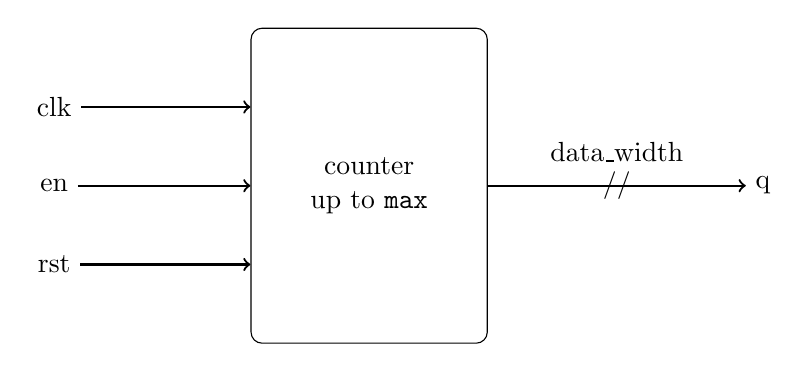
\begin{tikzpicture}[
        		decoration={
              		markings,
              		mark= at position 0.5 with {\node {//};}
              	}
            ]
            \tikzstyle{entity} = [rectangle, rounded corners, minimum width=3cm, minimum height=4cm,text centered, draw=black]
            \tikzstyle{arrow} = [thick,->]
            
           
            \node (counter)[entity, align=center]{counter  \\ up to \texttt{max}};
            \node(clk)[left of=counter, xshift = -3cm, yshift=1cm]{clk};
            \node(en)[left of=counter, xshift = -3cm, yshift=0cm]{en};
            \node(rst)[left of=counter, xshift = -3cm, yshift=-1cm]{rst};
            \node (q)[right of=counter, xshift = 4cm]{q};
            \draw [arrow] (clk.east) -- ([yshift=1cm]counter.west);
            \draw [arrow] (en.east) -- ([yshift=0cm]counter.west);
            \draw [arrow] (rst.east) -- ([yshift=-1cm]counter.west);
            \draw [arrow, postaction={decorate}] (counter.east) -- node[above=5pt] {data\_width} (q.west|-counter.east);
        \end{tikzpicture}
    \end{center}
    \caption{A Black Box Entity}
    \label{fig:bbe}
\end{figure}

\begin{figure}[H]
    \begin{center}
    	\lstinputlisting[language=VHDL, firstline=5, lastline=16]{../../src/counter.vhd}
    \end{center}
    \caption{A Black Box Entity in VHDL}
    \label{fig:bbe_vhdl}
\end{figure}

\subsubsection{White Box}
Now that the inputs and outputs are designed and implemented, we can look at the insides of the module. I have chosen to use a Moore Machine \footnote{\url{https://www.tutorialspoint.com/automata_theory/moore_and_mealy_machines.htm}} like in \cref{fig:mm}\footnote{\url{http://www-inst.eecs.berkeley.edu/~cs150/fa05/Lectures/07-SeqLogicIIIx2.pdf}} to do this. My implementation in \cref{fig:arch} should describe the logic diagram shown in \cref{fig:wbe}. Shown in \cref{fig:wbe} is a system whereby the output \texttt{q} is based on the current state output only, and not the current state plus some combination of the inputs, hence it's a \emph{Moore Machine}. There is a \emph{combinatorial logic} section which works out the next thing to get clocked into the register, and a \emph{synchronous} part which clocks that through and handles the advancement of the state.

\begin{figure}
    \begin{center}
        \includegraphics[width=\textwidth]{./src/moore_machine.png}
    \end{center}
    \caption{Generic Moore Machine}
    \label{fig:mm}
\end{figure}

\pgfdeclarelayer{background}
\pgfdeclarelayer{foreground}
\pgfsetlayers{background,main,foreground}

\begin{figure}
    \begin{center}
        \begin{tikzpicture}[
        		decoration={
             		markings,
              		mark= at position 0.7 with {\node {//};}
              	},
              	node distance = 0.5cm
            ]
            \tikzstyle{process} = [rounded corners, minimum width=2cm, minimum height=2cm, draw=black]
            \tikzstyle{arrow} = [thick,->]            
            
            \node (SL)[process,align=left]{
            	\begin{minipage}[t][3cm]{4cm} 
            		\fontsize{8pt}{8pt}\selectfont
            		\textbf{Synchronous Logic} \\ \\ \\ 
            		\texttt{if rising edge of clock:\\\hspace*{0.25cm}if rst = '1': \\ \hspace*{0.5cm}out = 0 \\\hspace*{0.25cm}else if en = '1': \\ \hspace*{0.5cm}out = in}
            	\end{minipage}
            };
            
            \node(clk)[left = of SL, xshift=-2cm, yshift=0.9cm]{clk};
            \node(en)[left = of SL, xshift=-2cm, yshift=0.3cm]{en};
            \node(rst)[left = of SL, xshift=-2cm, yshift=-0.3cm]{rst};
            \node(Q)[right= of SL, xshift=5cm]{q};

            \node (CL)[process, align=left, below = of SL,]{
            	\begin{minipage}[t][3cm]{4cm} 
            		\fontsize{8pt}{8pt}\selectfont
            		\textbf{Combinatorial Logic} \\ \\ \\
            		\texttt{if count + 1 $\geq$ max:\\\hspace*{0.25cm}count = 0 \\ else \\\hspace*{0.25cm}count = count + 1}
            	\end{minipage}
            };
            
            \draw [arrow]  ([xshift=1cm]SL.east) |- node[below]{count} (CL.east);
            \draw [arrow] (clk.east) -- ([yshift=0.9cm]SL.west);
            \draw [arrow] (en.east) -- ([yshift=0.3cm]SL.west);
            \draw [arrow] (rst.east) -- ([yshift=-0.3cm]SL.west);
            \draw [arrow] (CL.west) -| ([xshift=-1cm]CL.west) node[ below]{count} -- ([xshift=-1cm, yshift=-0.9cm]SL.west) -- node[left, above]{in} ([yshift=-0.9cm]SL.west);
            \draw [arrow, postaction={decorate}] (SL.east) -- node[xshift=-2.3cm,above] {out} node[xshift=1cm, above=5pt] {data\_width} (Q.west|-counter.east);


	\begin{pgfonlayer}{background}
               	\path (SL.north west)+(-2,0.2) node (a) {};
        		\path (CL.south east)+(+2.3,-0.2) node (b) {};
        		\path[rounded corners, draw, dashed] (a) rectangle (b);
    	\end{pgfonlayer}
	\end{tikzpicture}
    \end{center}
    \caption{A White Box Entity with pseudocode Moore Machine}
    \label{fig:wbe}
\end{figure}

\begin{figure}
    \begin{center}
    	\lstinputlisting[language=VHDL, firstline=18]{../../src/counter.vhd}
    \end{center}
    \caption{The White Box Entity in VHDL}
    \label{fig:arch}
\end{figure}

\begin{table}
    \begin{center}
    \begin{threeparttable}
        \begin{tabular}{| c | m{ 0.7\textwidth} |}
            \hline
             Keyword & Overview \\ \hline
             process & The start of a process, in a process each instructions happens sequentially \\ \hline
             signal & \handwaving Think of it as a wire that exists between processes. They are updated at the end of the process \\ \hline
             variable & \handwaving Variables can only exists in a process, they update immediately unlike signals \\ \hline
             architecture & Signifies the start of the internal details of an entity \\ \hline
             rising\_edge \tnote{*}& Syntactic sugar equivalent to 'if clk = '1' and clk'event' \\ \hline
        \end{tabular}
        \begin{tablenotes}
        \footnotesize
        \item[*] Not really a keyword, but important to know.
        \end{tablenotes}
        \end{threeparttable}
        \caption{An overview of keywords we have seen}
        \label{table:keywords}
    \end{center}
\end{table}



\begin{table}[H]
    \begin{center}
    \begin{threeparttable}
        \begin{tabular}{| c | m{ 0.7\textwidth} |}
            \hline
             Data Type & Overview \\ \hline
             std\_ulogic \tnote{*}& This is defined in the ieee.std\_logic\_1164 package and is an enumeration with the values 'U', 'X', '0', '1', 'Z', 'W', 'L', 'H' and '-' \\ \hline
             std\_ulogic\_vector & Again defined in the ieee.std\_logic\_1164 package this is an array of std\_ulogics \\ \hline
             positive & This is a VHDL standard type and it's an integer with a range of 1 to at least $2^{31} -1$  \\ \hline
             record & This is a VHDL standard type, similar to a struct \\ \hline
        \end{tabular}
        \begin{tablenotes}
        \footnotesize
        \item[*] Many online examples use std\_logic, this is the 'resolved' version of std\_ulogic. They are effectively the same except a signal of type std\_logic can be controlled from different places and errors will only show themselves at runtime.
        \end{tablenotes}
        \end{threeparttable}
        \caption{An overview of data types we have seen}
        \label{table:datatypes}
    \end{center}
\end{table}

%------------------------------------------------------------------------------------------------------------------------------------------------------
\subsection{How to get started with a new design}
There are heaps of tutorials online for how to do this in all sorts of toolchains, such as \url{https://reference.digilentinc.com/vivado/getting_started/start} or \url{https://www.intel.com/content/www/us/en/programmable/documentation/yoq1529444104707.html} so I won't cover that here. If you're reading this and it's printed then good luck typing those in! Ask me for an electronic copy and I'll make sure you get one, alternatively google \emph{Quartus getting started} or similar.

\subsection{How to see output from our VHDL}
There are two ways to do this
\begin{enumerate}
    \item \textbf{Simulation} - this is often the quickest method as it allows us to delve into every signal and process of our design. This also happens on our development machine so we can make great progress and do 95\% of our coding without a device.
    \item \textbf{Putting on the hardware} - this is where stuff gets tough. In this step the design will run at full speed on a device. You should only be doing this when you feel sufficiently confident that it'll work. If anything goes wrong here it can be extremely tough to debug it, or even detect it! 
\end{enumerate}
\subsubsection{Simulation}
Simulations can be stimulated via a test bench (my personal favourite) or manually in some simulators. For this tutorial I have created a testbench to do this
How to interpret the waveforms
\subsubsection{On the hardware itself}
How to load onto the board

\section{Further Activities}
If this has been fun, and you want to learn more here are some useful resources I have had successes with:

\begin{itemize}
    \item Effective Coding with VHDL\footnote{\url{https://www.amazon.co.uk/Effective-Coding-VHDL-Principles-Practice/dp/0262034220}} 
    \item Awesome VHDL \footnote{\url{https://github.com/VHDL/awesome-vhdl}}
    \item Digital Fundamentals \footnote{\url{https://www.amazon.co.uk/Digital-Fundamentals-Thomas-L-Floyd/dp/0132737965}}
\end{itemize}

\end{document}
